\newpage
\section{Large and Fast: Exploiting Memory Hierarchy}
\subsection{Large and Fast}
\begin{itemize}\small
    \item Size large enough to store any program (Turing Completeness)
    \item Speed fast enough to catch up with the speed of the processor (IF, MEM....)
\end{itemize}

Reality: we don’t have an ideal memory, so we need a hierarchical design. 

\subsubsection{Key merits of a memory}
\begin{enumerate}\small
    \item Speed
    \subitem Physical cell property
    \subitem Access schemes
    \item Cost per bit (cost vs size)
    \item Volatility
    \item Endurance cycles
    \subitem Controller design
\end{enumerate}

\subsubsection{Memory Technologies}
Memories: Review
\begin{enumerate}\small
    \item SRAM (Static Random Access Memory)
    \begin{itemize}
        \item value is stored on a pair of inverting gates
        \item very fast but takes up more space than DRAM
    \end{itemize}
    \begin{figure}[!htb]
        \centering
        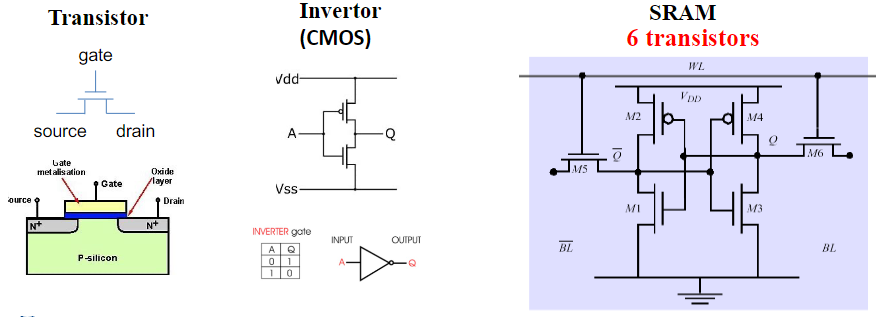
\includegraphics[width=0.42\textwidth]{CO5/SRAM}
        \caption{SRAM}
    \end{figure}
    \item DRAM (Dynamic Random Access Memory)
    \begin{itemize}
        \item Value is stored as a charge on capacitor
        \item Very small but slower than SRAM (factor of 5 to 10)
        \item Must periodically be refreshed
        \item Read contents and write back (destructive read)
    \end{itemize}
    \begin{figure}[!htb]
        \centering
        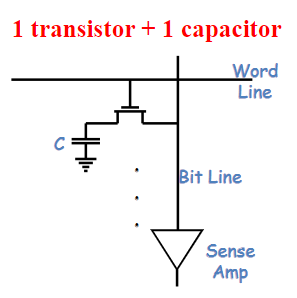
\includegraphics[width=0.209\textwidth]{CO5/DRAM}
        \caption{DRAM}
    \end{figure}
    \subitem Advanced DRAM Organization: 
    \begin{itemize}
        \item Bits in a DRAM are organized as a rectangular array
        \subitem DRAM accesses an entire row
        \subitem Burst mode: supply successive words from a row with reduced
        latency (SDRAM)
        \item Double data rate (DDR) DRAM
        \subitem Transfer on rising and falling clock edges
        \item Quad data rate (QDR) DRAM
        \subitem Separate DDR inputs and outputs
    \end{itemize}
    \begin{figure}[!htb]
        \centering
        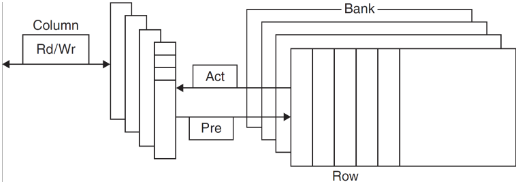
\includegraphics[width=0.309\textwidth]{CO5/Advanced DRAM Organization}
        \caption{Advanced DRAM Organization}
    \end{figure}
    \item Flash Storage (Nonvolatile semiconductor storage)
    \begin{itemize}
        \item 100x – 1000x faster than disk
        \item Smaller, lower power, more robust
        \item But more \$/GB than disk (between disk andDRAM)
    \end{itemize}
    \subitem Flash Types
    \begin{itemize}
        \item  NOR flash: bit cell like a NOR gate
        \subitem Random read/write access
        \subitem Used for instruction memory in embedded systems
        \item NAND flash: bit cell like a NAND gate
        \subitem Denser (bits/area), but block-at-a-time access
        \subitem Cheaper per GB
        \subitem Used for USB keys, media storage, ...
        \item Flash bits wears out after 10000's of accesses
        \subitem Not suitable for direct RAM or disk replacement
        \subitem Wear leveling: remap data to less used blocks
    \end{itemize}
    \begin{figure}[!htb]
        \centering
        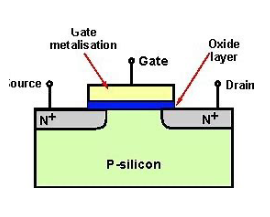
\includegraphics[width=0.2\textwidth]{CO5/Flash Storage}
        \caption{Flash Storage}
    \end{figure}
    \begin{figure}[!htb]
        \centering
        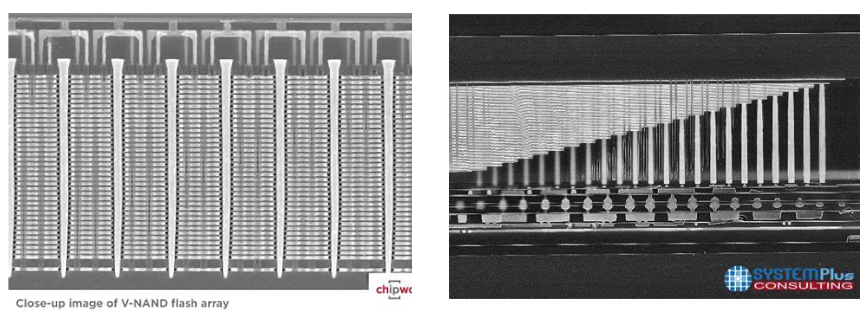
\includegraphics[width=0.42\textwidth]{CO5/3D flash makes SSD low cost and faster}
        \caption{3D flash makes SSD low cost and faster}
    \end{figure}
    \item Disk Storage (Nonvolatile, rotating magnetic storage)
    \begin{figure}[!htb]
        \centering
        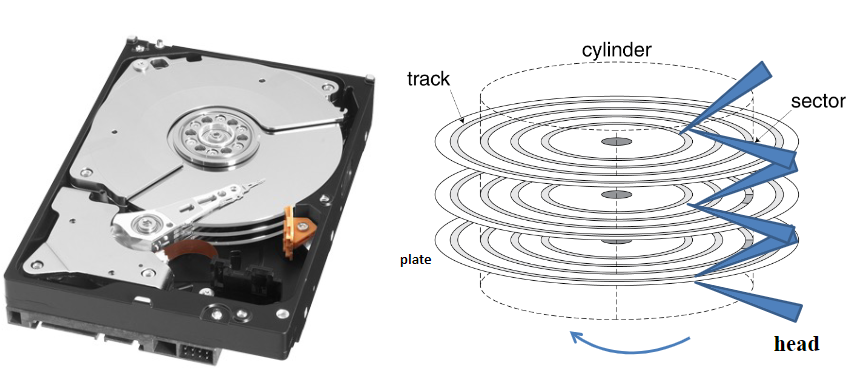
\includegraphics[width=0.309\textwidth]{CO5/Disk Storage}
        \caption{Disk Storage}
    \end{figure}
    \subitem Disk Sectors and Access
    \begin{itemize}
        \item Each sector records
        \subitem Sector ID
        \subitem Data (512 bytes, 4096 bytes proposed)
        \subitem Error correcting code (ECC): Used to hide defects and recording errors
        \item Access to a sector involves
        \subitem Queuing delay if other accesses are pending
        \subitem Seek: move the heads
        \subitem Rotational latency
        \subitem Data transfer
        \subitem Controller overhead        
    \end{itemize}
    rpm(round per minute)
\end{enumerate}

\subsection{Memory Hierarchy Introduction}
\begin{enumerate}\small
    \item Temporal locality: Items accessed recently are likely to be accessed again soon.
    \item Spatial locality: Items near those accessed recently are likely to be accessed soon
\end{enumerate}

\subsubsection{Taking Advantage of Locality}
\begin{enumerate}\small
    \item Memory hierarchy
    \item Store everything on disk
    \item Copy recently accessed (and nearby) items from disk to smaller DRAM memory
    \subitem Main memory
    \item Copy more recently accessed (and nearby) items from DRAM to smaller SRAM memory
    \subitem Cache memory attached to CPU
\end{enumerate}

\begin{figure}[!htb]
    \centering
    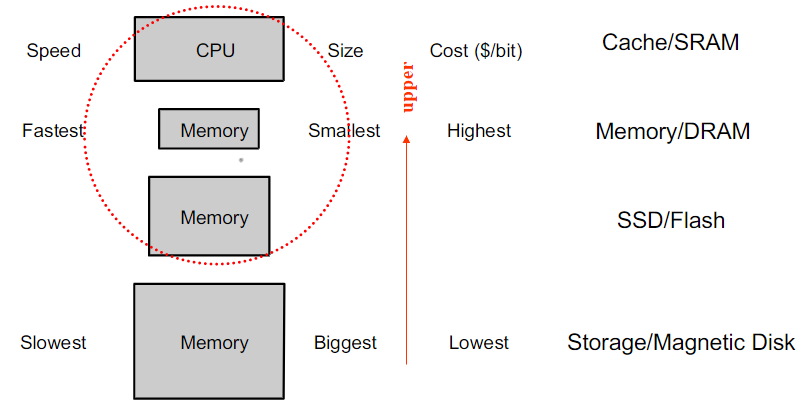
\includegraphics[width=0.42\textwidth]{CO5/Memory Hierarchy Levels}
    \caption{Memory Hierarchy Levels}
\end{figure}

\subsubsection{Some important items}
\begin{enumerate}\small
    \item Hit: The CPU accesses the upper level and succeeds.
    \subitem Hit ratio: hits/accesses
    \item Miss: The CPU accesses the upper level and fails.
    \subitem Time taken: miss penalty
    \subitem Miss ratio: misses/accesses$= 1 – $hit ratio
    \item Hit time: The time to access the upper level of the memory hierarchy, which includes the time needed to determine whether the access is a hit or a miss.
    \item miss penalty: The time to replace a block in the upper level with the corresponding block from the lower level, plus the time to deliver this block to the processor.
\end{enumerate}


\subsubsection{Exploiting Memory Hierarchy}
The method
\begin{enumerate}\small
    \item Hierarchies bases on memories of different speeds and size
    \item The more closely CPU the level is,the faster the one is.
    \item The more closely CPU the level is,the smaller the one is.
    \item The more closely CPU the level is,the more expensive. 
\end{enumerate}

\begin{figure}[!htb]
    \centering
    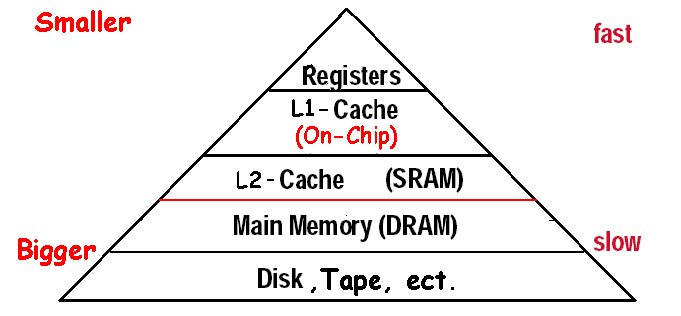
\includegraphics[width=0.309\textwidth]{CO5/Memory Hierarchy}
    \caption{Levels in the Memory Hierarchy}
\end{figure}

\subsection{The basics of Cache}
\subsubsection{Simple implementations}

\begin{figure}[!htb]
    \centering
    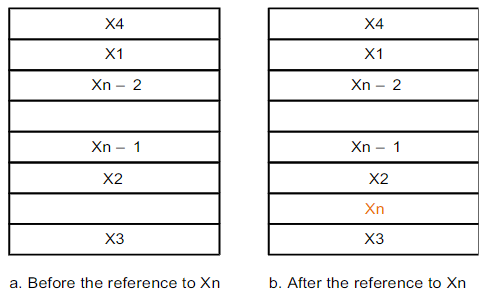
\includegraphics[width=0.24\textwidth]{CO5/Simple implementations}
    \caption{Simple implementations}
\end{figure}

For each item of data at the lower level, there is exactly one location in the cache where it might be.

Two issues:
\begin{itemize}
    \item  How do we know if a data item is in the cache?
    \item  If it is, how do we find it?
\end{itemize}

Our first example: ``direct mapped''. 

\subsubsection{Direct Mapped Cache}
\begin{figure}[!htb]
    \centering
    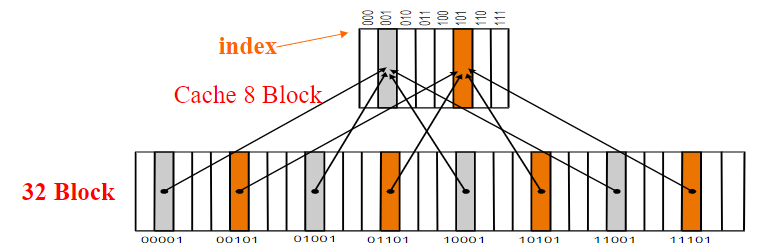
\includegraphics[width=0.42\textwidth]{CO5/Direct Mapped Cache}
    \caption{Direct Mapped Cache}
    \label{Direct Mapped Cache}
\end{figure}

Direct-mapping algorithm: (Block address) modulo (Number of blocks in the cache). 

Fortunately, while the cache has $2^n$ blocks, the corresponding index is equal to the lowest $n$ bits of memory block address. In \textbf{Figure} \ref{Direct Mapped Cache}, $n=3$.

\paragraph{Tags and Valid Bits}
To know which particular block is stored in a cache location: 
\begin{enumerate}\small
    \item Store block address as well as the data
    \item Actually, only need the high-order bits
    \item Called the tag
\end{enumerate}

If there is no data in a location:
\begin{itemize}\small
    \item Valid bit: $1 =$ present, $0 =$ not present
    \item Initially 0
\end{itemize}

\paragraph{Accessing a cache}
Memory block address is larger than cache block address. 

\begin{figure}[!htb]
    \centering
    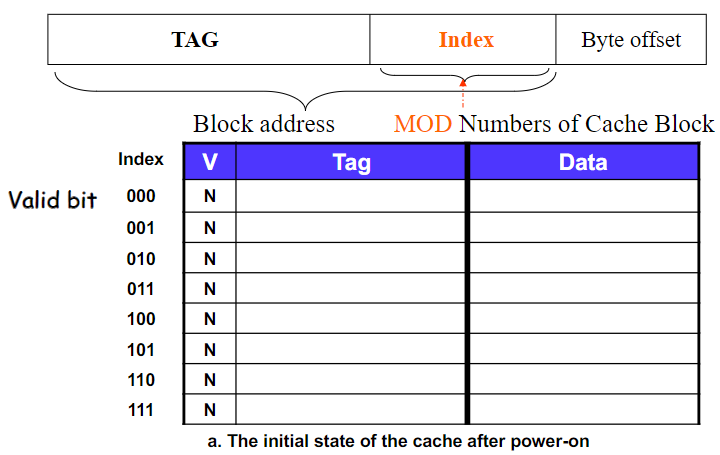
\includegraphics[width=0.42\textwidth]{CO5/Accessing a cache}
    \caption{Accessing a cache}
\end{figure}

\paragraph{Direct Mapped Cache Construction}

\begin{figure}[!htb]
    \centering
    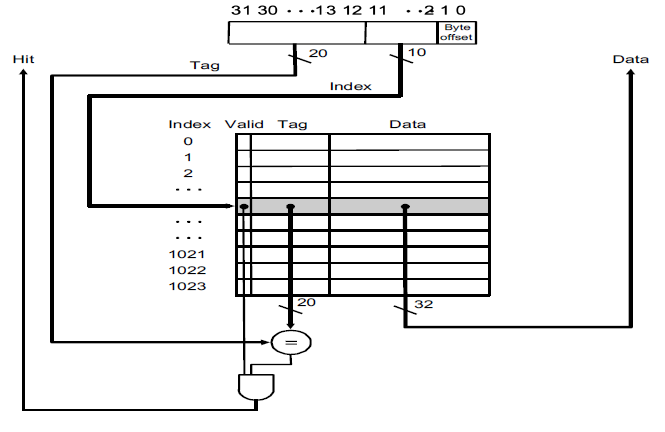
\includegraphics[width=0.42\textwidth]{CO5/Direct Mapped Cache Construction}
    \caption{Direct Mapped Cache Construction}
\end{figure}


\begin{itemize}\small
    \item Tag bits: $32-(n+m+2)$
    \item Cache size: $2^n$
    \item Index to reference words in block: $m$
    \item Total cache size: $2^n \times (\text{block size}+\text{tag size}+\text{valid bit})$
\end{itemize}

\paragraph{Bits in Cache}Example:

How many total bits are required for a direct-mapped cache 16KB of data and 4-word blocks, assuming a 32-bit address?

Answer: {\small
    \begin{align*}
        1 \text{word}&=32 \text{bits}=4 \text{bytes}\\
        16KiB&=4K \text{words}=2^{12} \text{words}\\
        1 \text{block}&=4 \text{words}=16\text{bytes}\\
        \text{index bits}&=\frac{2^{12}}{2^2}=2^{10}\text{blocks}\\
        \text{Tag bits}&=\text{address}-\text{index}-\text{block size}-\text{byte offset}\\
        &=32-10-2-2=18\text{bits}\\
        \text{Valid bit}&=1 \text{bit}\\
        \text{Total Cache size}&=2^{10}(16*8+18+1)=147K\text{bits}
    \end{align*}
}
It is about $\frac{147}{128}\approx 1.15$ times as many as needed just for the data. 

\begin{figure}[!htb]
    \centering
    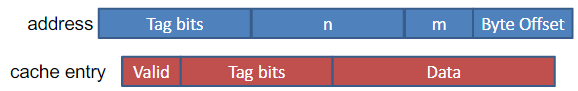
\includegraphics[width=0.42\textwidth]{CO5/Bits in Cache}
    \caption{Bits in Cache}
\end{figure}

% \paragraph{Mapping an Address to Multiword Cache Block}
% Example: 
% P35


\paragraph{Handling Cache reads hit and Misses}\quad 

Read hits

Read misses—two kinds of misses
\begin{itemize}\small
    \item instruction cache miss
    \subitem When an instruction cache miss: 
    \begin{enumerate}
        \item Stall the CPU, 
        \item fetch block from memory, 
        \item deliver to cache, 
        \item restart CPU read
    \end{enumerate}
    \item data cache miss
\end{itemize}

Write hits: Difference Strategy
\begin{itemize}\small
    \item write-back: Cause Inconsistent
    \subitem Wrote the data into only the data cache
    \subitem Strategy --- write back data from the cache to memory later
    \subitem Fast!
    \item  write-through: Ensuring Consistent
    \subitem Write the data into both the memory the cache
    \subitem Strategy --- writes always update both the cache and the memory
    \subitem Slower! --- can use write buffer to speed up 
\end{itemize}

Write misses: read the entire block into the cache, then write the word. 

\subsubsection{Four Questions for Memory Hierarchy Designers}
\textbf{Caching} is a general concept used in processors, operating systems, file systems, and applications.
\begin{enumerate}\small
    \item Q1: Where can a block be placed in the upper level? (Block placement)
    \subitem Fully Associative, Set Associative, Direct Mapped
    \item Q2: How is a block found if it is in the upper level? (Block identification)
    \subitem Tag/Block
    \item Q3: Which block should be replaced on a miss? (Block replacement)
    \subitem Random, LRU,FIFO
    \item Q4: What happens on a write? (Write strategy)
    \subitem Write Back or Write Through (with Write Buffer)
\end{enumerate}

\paragraph{Q1: Block Placement}
\begin{itemize}
    \item Direct mapped: Usually address MOD Number of blocks in cache
    \item Fully associative: Block can go anywhere in cache
    \item Set associative: Block can go in one of a set of places in the cache
\end{itemize}
Note that direct mapped is the same as 1-way set associative, and fully associative is m-way set-associative (for a cache with m blocks).

\begin{figure}[!htb]
    \centering
    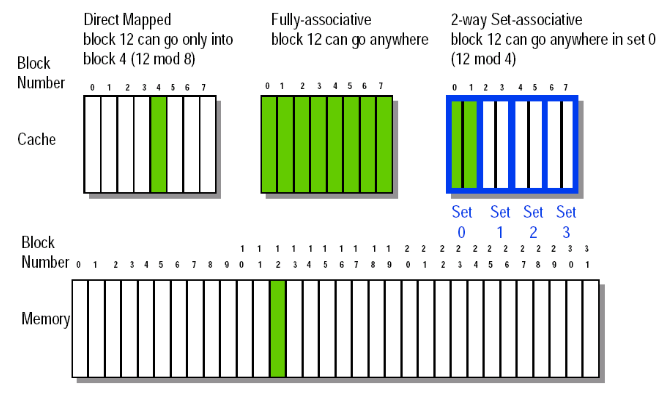
\includegraphics[width=0.42\textwidth]{CO5/8-32 Block Placement}
    \caption{8-32 Block Placement}
\end{figure}

\paragraph{Q2: Block Identification}
\begin{itemize}
    \item Tag: As a part of the address differentiation block
    \item Valid bit:  tells if the contents of the cache block are valid
\end{itemize}

The Format of the Physical Address: 
\begin{itemize}
    \item Tag
    \item Index
    \subitem {\small The set, in case of a set-associative cache}
    \subitem {\small The block, in case of a direct-mapped cache}
    \item Block Offset: {\small used to search for the word in 1 block, in case of a set-associative cache.}
    \item Byte Offset: {\small used to search for the bytes in 1 word.}
\end{itemize}
{\small
    \begin{align*}
        \text{address size}=\text{Tag size}+\text{index size}+\text{block offset}+\text{byte offset}
    \end{align*}
}

% 44-46 example pic 

\paragraph{Q3: Block Replacement}
\begin{itemize}
    \item In a direct-mapped cache, there is only one block that can be replaced
    \item In set-associative and fully-associative caches, there are N blocks (where N is the degree of associativity)
\end{itemize}

Strategy of Block Replacement:
\begin{enumerate}
    \item Random replacement: {\small randomly pick any block}
    \item Least-recently used (LRU): {\small pick the block in the set which was least recently accessed}
    \item First in,first out(FIFO): {\small Choose a block from the set which was first came into the cache}
\end{enumerate}

\paragraph{Q4: Write Strategy}
\begin{itemize}
    \item Write-through cache: {\small the data is written to memory}
    \subitem Advanced: {\small Read misses don't result in writes, memory hierarchy is consistent and it is simple to implement.}
    \item Write-back cache: {\small the data is NOT written to memory}
    \subitem Advantage: {\small Writes occur at speed of cache and main memory bandwidth is smaller when multiple writes occur to the same block.}
\end{itemize}

Write stall: When the CPU must wait for writes to complete during write through. 

Write buffers: A small cache that can hold a few values waiting to go to main memory. This buffer helps when writes are clustered.

\begin{figure}[!htb]
    \centering
    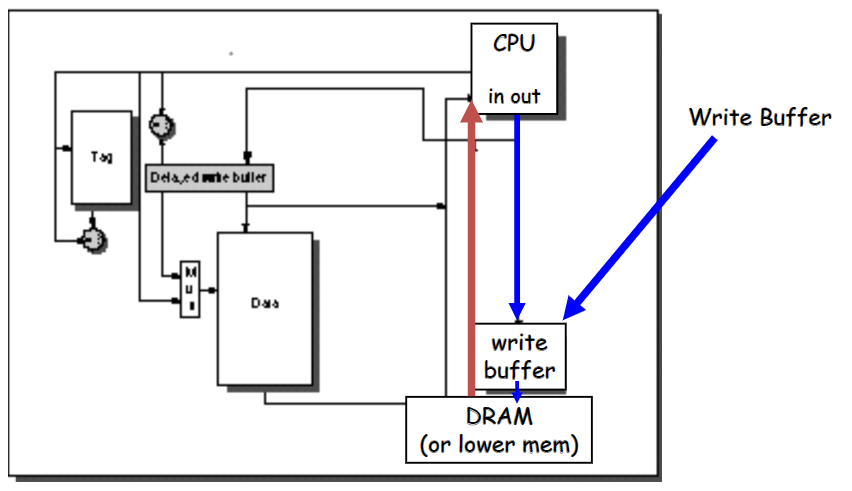
\includegraphics[width=0.309\textwidth]{CO5/Write buffers}
    \caption{Write buffers}
\end{figure}

Write misses: If a miss occurs on a write (the block is not present), there are two options
\begin{enumerate}
    \item Write allocate: {\small The block is loaded into the cache on a miss before anything else occurs.}
    \item Write around (no write allocate): {\small The block is only written to main memory. It is not stored in the cache.}
\end{enumerate}
In general, write-back caches use write-allocate , and write-through caches use write-around .

\subsubsection{Designing the Memory system to Support Cache}
Taking advantage of spatial locality to lower miss rates with many word in the block \ref{Larger blocks exploit spatial locality}. 
\begin{figure}[!htb]
    \centering
    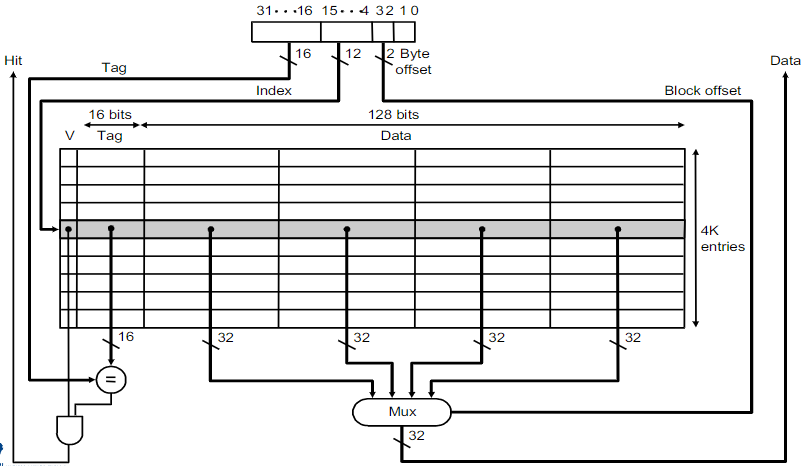
\includegraphics[width=0.42\textwidth]{CO5/Larger blocks exploit spatial locality}
    \caption{Larger blocks exploit spatial locality}
    \label{Larger blocks exploit spatial locality}
\end{figure}

Make reading multiple words easier by using banks of memory \ref{Different memory system}.

\begin{figure}[!htb]
    \centering
    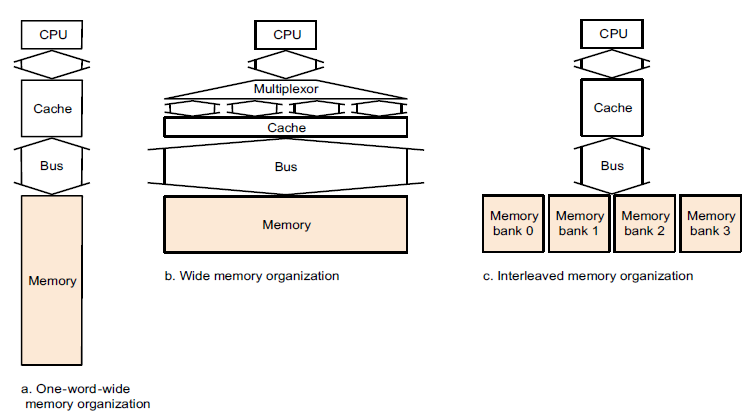
\includegraphics[width=0.42\textwidth]{CO5/the Memory system}
    \caption{Different memory system}
    \label{Different memory system}
\end{figure}

\paragraph{Performance in different block size}
Increasing the block size tends to decrease miss rate \ref{Performance in different block size}.
\begin{figure}[!htb]
    \centering
    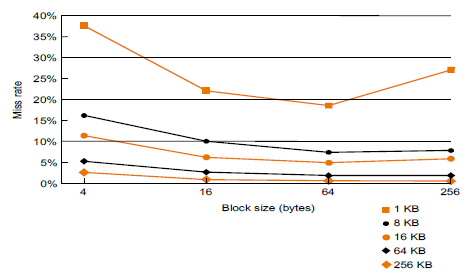
\includegraphics[width=0.42\textwidth]{CO5/Performance in different block size}
    \caption{Performance in different block size}
    \label{Performance in different block size}
\end{figure}

\subsection{Measuring and improving cache performance}
Discuss two questions:
\begin{enumerate}\small
    \item How to measure cache performance?
    \item How to improve performance?
\end{enumerate}

The main contents are the following:
\begin{enumerate}\small
    \item Measuring cache performance
    \item Reducing cache misses by more flexible placement of blocks
    \item Reducing the miss penalty using multilevel caches
\end{enumerate}
{\small
    \begin{align*}
        &\text{ Average Memory Assess Time (AMAT)}\\
        =& \text{ hit time} + \text{miss time}\\
        =& \text{ hit time} + \text{miss rate} \times \text{miss penalty}
    \end{align*}
}
\begin{itemize}\small
    \item Hit time: The time to access the upper level of the memory hierarchy, which includes the time needed to determine whether the access is a hit or a miss.
    \item Miss penalty: The time to replace a block in the upper level with the corresponding block from the lower level, plus the time to deliver this block to the processor.
\end{itemize}

\subsubsection{Measuring cache performance}
We use CPU time to measure cache performance. 
{\small
Before
\begin{align*}
    \text{CPU}_{\text{time}}=\text{I}\times \text{CPI} \times \text{clock cycle time}
\end{align*}
And now
\begin{align*}
    &\text{ CPU time}\\
    =& \text{ CPU execution clock cycles} +\text{Memory-stall clock cycles}\\
    &\text{ Memory-stall clock cycles}\\
    =&\text{ \# of mem instructions}\times \text{miss ratio}\times \text{miss penalty} \\
    =&\text{ Read-stall cycles} + \text{Write-stall cycles}
\end{align*}
For Read-stall
\begin{align*}
    &\text{ Read-stall cycles}\\
    =& \frac{\text{\# of Read}}{\text{Program}}\times \text{Read miss rate}\times \text{Read miss penalty}
\end{align*}
For a write-through plus write buffer schemes:
\begin{align*}
    &\text{ Write-stall cycles}\\
    =& \frac{\text{\# of Write}}{\text{Program}}\times \text{Write miss rate}\times \text{Write miss penalty}\\
    &+\text{Write buffer stalls}
\end{align*}

}
Note that
\begin{itemize}\small
    \item If the write buffer stalls are small, we can safely ignore them .
    \item If the cache block size is one word, the write miss penalty is 0.
\end{itemize}

\paragraph{Combine the reads and writes}{
    \small
    In most write-through cache organizations, the read and write miss penalties are the same, the time to fetch the block from memory. (这个表述不完全正确)

    If we neglect the write buffer stalls, we get the following equation:
    \begin{align*}
        &\text{ Memory-stall clock cycles}\\
        =& \frac{\text{Memory accesses}}{\text{Program}}\times \text{Miss rate}\times \text{Miss penalty}
    \end{align*}
    We can also write this as:
    \begin{align*}
        &\text{ Memory-stall clock cycles}\\
        =& \frac{\text{instructions}}{\text{Program}}\times \frac{\text{Misses}}{\text{instructions}}\times \text{Miss penalty}
    \end{align*}
}

\subsubsection{Calculating cache performance}
Assume:
\begin{itemize}\small 
    \item instruction cache miss rate 2\%
    \item data cache miss rate 4\%
    \item CPI without any memory stalls 2
    \item miss penalty 100 cycles
    \item The frequency of all loads and stores in gcc is 36\%
\end{itemize}

Question: How faster a processor would run with a perfect cache? 

Answer:{
    \small
    \begin{align*}
        \text{Instruction miss cycles}&=I\times2\%\times100=2.00I\\
        \text{Data miss cycles}&=I\times 36\%\times 4\%\times 100=1.44I\\
        \text{Total memory-satll cycles}&=2.00I+1.44I=3.44I
    \end{align*}
    \begin{align*}
        \text{CPI with stall}&=\text{CPI with perfect cache}+\text{Total memory-stalls}\\
        &=(2+3.44)I=5.44I
    \end{align*}
    \begin{align*}
        \frac{\text{CPU time with stalls}}{\text{CPU time with perfect cache}}&=\frac{I\times \text{CPI}_{\text{stall}}\times \text{Clock cycle}}{I\times \text{CPI}_{\text{perfect}}\times \text{Clock cycle}}\\
        &=\frac{\text{CPI}_{\text{stall}}}{\text{CPI}_{\text{perfect}}}=\frac{5.44}{2}=2.72
    \end{align*}
}
\paragraph{What happens if the processor is made faster}
Assume CPI reduces from 2 to 1. {
    \small
    \begin{align*}
        \text{CPI with stall}&=\text{CPI with perfect cache}+\text{Total memory-stalls}\\
        &=(1+3.44)I=4.44I
    \end{align*}
    \begin{align*}
        \frac{\text{CPU time with stalls}}{\text{CPU time with perfect cache}}
        &=\frac{\text{CPI}_{\text{stall}}}{\text{CPI}_{\text{perfect}}}=\frac{4.44}{1}=4.44
    \end{align*}

    Ratio time for Memory stalls from $\frac{3.44}{5.44}=63\%$ to $\frac{3.44}{4.44}=77\%$
}

\paragraph{With Increased Clock Rate}
{\small Suppose we increase the performance of the computer in the previous example by doubling its clock rate for same memory system.}

Question : How much faster will the computer be with the faster clock to slow clock?

Answer:{
    \small
    \begin{align*}
        \text{Total CPI}&=(2\%\times 200)+36\%(4\%\times200)=6.88\\
        \text{CPI with cache miss}&=2+6.88=8.88
    \end{align*}
    \begin{align*}
        \frac{\text{Performance with fast clock}}{\text{Performance with slow clock}}&=\frac{\text{Execution time with slow clock}}{\text{Execution time with fast clock}}\\
        &=\frac{I\times \text{CPI}_{\text{slow clock}}\times \text{Clock cycle}}{I\times \text{CPI}_{\text{fast clock}}\times \text{Clock cycle}/2}\\
        &=\frac{5.44}{8.88/2}=1.23
    \end{align*}
    This, the computer with the faster clock is about 1.2 times faster rather than 2 time faster.
}

\subsubsection{Solution: Reducing cache misses by more flexible placement of blocks}
\begin{enumerate}\small
    \item The disadvantage of a direct-mapped cache
    \item The basics of a set-associative cache
    \item Miss rate versus set-associative
    \item Locating a block in the set-associative cache
    \item Size of tags versus set associative
    \item Choosing which block to replace
\end{enumerate}

\paragraph{The basics of a set-associative cache}
Decreasing miss ratio with associativity. 

A set-associative cacheis divided into some sets. A set contains several blocks. A memory block is mapped to a set in the cache. The mapping algorithm is:{\tiny
\begin{align*}
    \text{Set number (Index)}=\text{Memory block number}\%\text{Number of sets in the cache}
\end{align*}
}{\small
\begin{itemize}
    \item If a set has only one block, this set-associative cache is actually a direct-mapped cache.
    \item If a set-associative cache has only one set, this set-associative cache is called a fully-associative cache.
\end{itemize}
}

\begin{figure}[!htb]
    \centering
    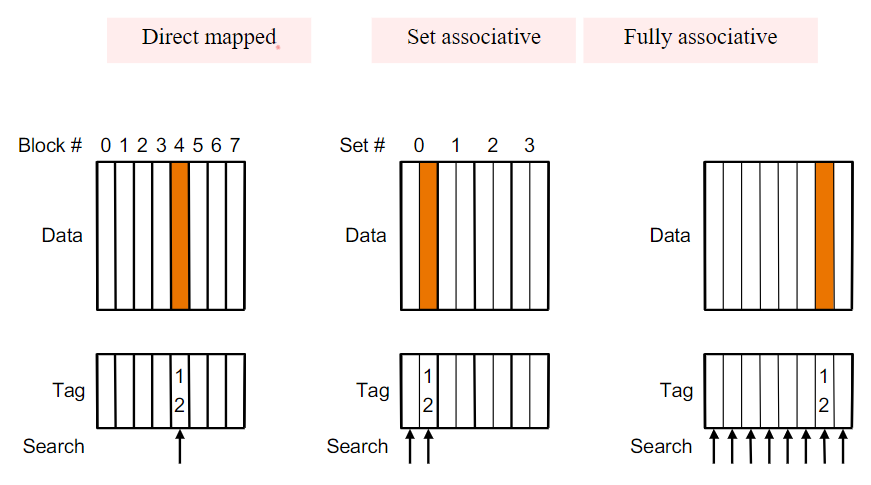
\includegraphics[width=0.42\textwidth]{CO5/Memory block whose address is 12 in a cache with 8 blocks for different mapped}
    \caption{Memory block whose address is 12 in a cache with 8 blocks for different mapped}
\end{figure}


\paragraph{Locating a block in the set-associative cache}
\begin{figure}[!htb]
    \centering
    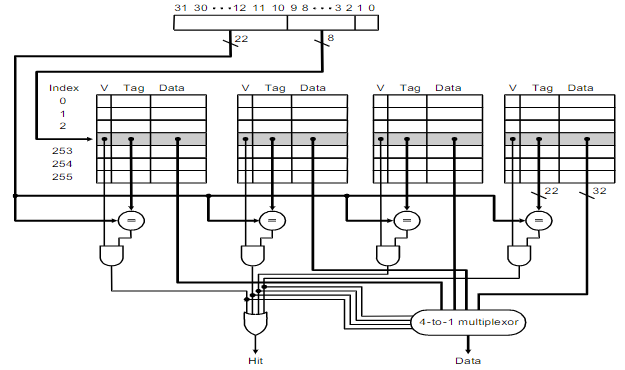
\includegraphics[width=0.42\textwidth]{CO5/Locating a block in the set-associative cache}
    \caption{Locating a block in the set-associative cache}
    \label{Locating a block in the set-associative cache}
\end{figure}
The implementation of a four-way set-associative cache requires four comparators and a 4-to-1 multiplexor \textbf{Figure} \ref{Locating a block in the set-associative cache}.

\paragraph{Size of tags versus set associativity}
Assume:
\begin{itemize}\small
    \item Cache size is 4K blocks
    \item Block size is 4 words
    \item Physical address is 32 bits
\end{itemize}

Question: Find the total number of set and total number of tag bits for variety associativity. 

Answer:{\small
    \begin{align*}
        \text{Offset size}&=4\text{word}\times 4\text{byte/word}=16\text{byte}=2^4
    \end{align*}
    \begin{itemize}
        \item For direct-mapped
        \begin{align*}
            \text{Number of cache block}&=2^{12}\\
            \text{Bit of Tag}&=(32-4-12)\times 4K=64K\text{bits}
        \end{align*}
        \item For 2-way associative
        \begin{align*}
            \text{Number of cache block}&=2^{11}\\
            \text{Bit of Tag}&=(32-4-11)\times 4K=67K\text{bits}
        \end{align*}
        \item For 4-way associative
        \begin{align*}
            \text{Number of cache block}&=2^{10}\\
            \text{Bit of Tag}&=(32-4-10)\times 4K=72K\text{bits}
        \end{align*}
        \item For full associative
        \begin{align*}
            \text{Number of cache block}&=1\\
            \text{Bit of Tag}&=(32-4)\times 4K=112K\text{bits}
        \end{align*}
    \end{itemize}
}

\paragraph{Choosing which block to replace}
Least recently used (LRU): the block replaced is the one that has been unused for the longest time.

\subsubsection{Decreasing miss penalty with multilevel caches}
Add a second level cache:
\begin{itemize}\small
    \item often primary cache is on the same chip as the processor
    \item use SRAMs to add another cache above primary memory (DRAM)
    \item miss penalty goes down if data is in 2nd level cache
\end{itemize}

Example: 
\begin{itemize}\small
    \item CPI of 1.0 on a 5GHz machine with a 2\% miss rate, 100ns DRAM access
    \item Adding 2nd level cache with 5ns access time decreases miss rate to 0.5\%
\end{itemize}{\small
    The CPI with one level of caching:
    \begin{align*}
        \text{Miss penalty to main memory}&=100\times10^{-9}\text{s}\times5\times10^9\text{Hz}\\
        &=500\text{clock cycles}\\
        \text{Total CPI}&=1+\text{Memory-stall CPI}\\
        &=1+2\%\times 500=11
    \end{align*}

    The CPI with Two level of cache:
    \begin{align*}
        \text{Miss penalty with levels of cache}&=5\times5\\
        &=25\text{clock cycles}\\
        \text{Total CPI}&=1+\text{Primary stalls CPI}\\
        &\ \ +\text{Secondary stalls CPI}\\
        &=1+2\%\times 25+0.5\%\times 500=4
    \end{align*}

    The processor with secondary cache is faster by $\frac{11}{4}=2.8$
}
Using multilevel caches:
\begin{itemize}\small
    \item try and optimize the hit time on the 1st level cache
    \item try and optimize the miss rate on the 2nd level cache
\end{itemize}

\subsubsection{Miss Penalties (Include Write-back Cache)}
\begin{figure}[!htb]
    \centering
    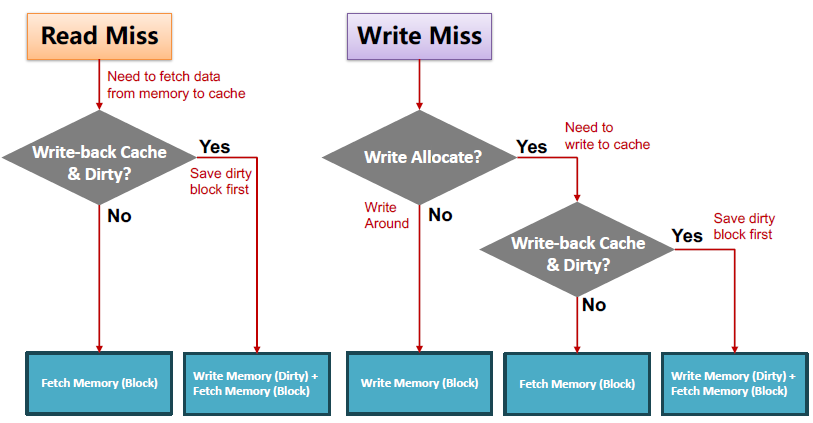
\includegraphics[width=0.42\textwidth]{CO5/Miss Penalties}
    \caption{Miss Penalties}
\end{figure}
If the write buffer stalls are small, we can safely ignore them. (No penalty on Write Memory)

\subsection{Virtual Memory}
Main Memory act as a ``Cache'' for the secondary storage. Motivation:
\begin{itemize}\small
    \item Efficient and safe sharing of memory among multiple programs.
    \item  Remove the programming burdens of a small, limited amount of main memory.
\end{itemize}
Translation of a program's address space to physical address. 

\begin{figure}[!htb]
    \centering
    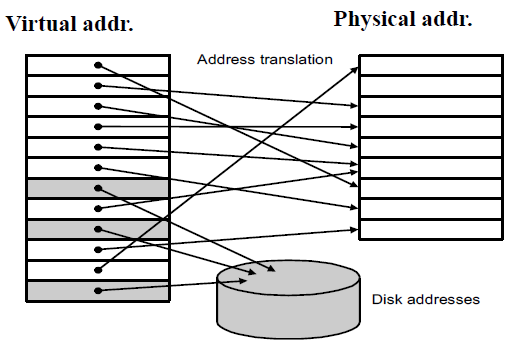
\includegraphics[width=0.42\textwidth]{CO5/Main memory can act as a cache for the secondary storage (disk)}
    \caption{Main memory can act as a cache for the secondary storage (disk)}
\end{figure}
Advantages:
\begin{itemize}\small
    \item illusion of having more physical memory
    \item program relocation
    \item protection
\end{itemize}

\subsubsection{Pages: virtual memory blocks}
The number of virtual pages is larger than physical pages. 

Page faults (miss): the data is not in memory, retrieve it from disk

\begin{figure}[!htb]
    \centering
    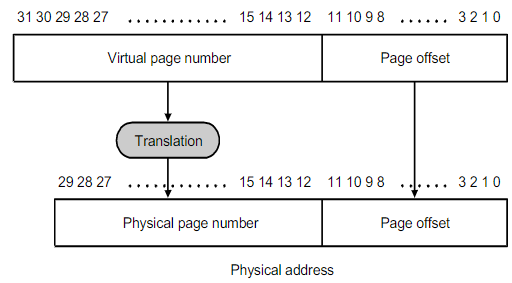
\includegraphics[width=0.309\textwidth]{CO5/virtual memory blocks}
    \caption{virtual memory blocks}
\end{figure}

\subsubsection{Page Tables}
\begin{enumerate}\small
    \item Virtual to physical address. 
    \item Stored into the memory, indexed by the virtual page number
    \item Each Entry in the table contains the physical page number for that virtual pages if the page is current in memory
    \item Page table, Program counter and the page table register, specifies the state of the program. Each process has one page table.
\end{enumerate}

\begin{figure}[!htb]
    \centering
    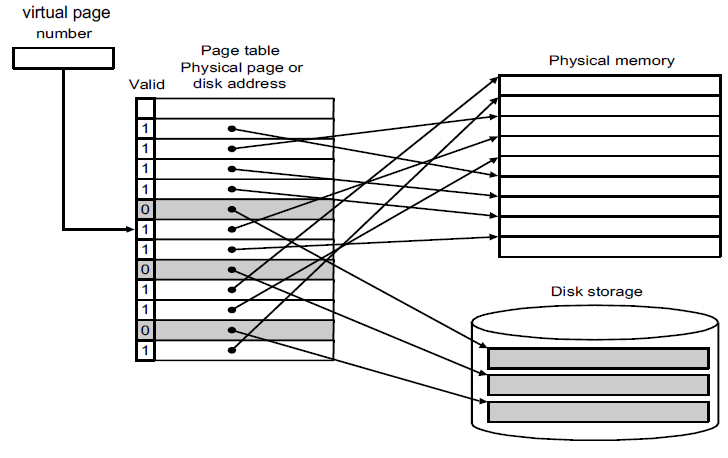
\includegraphics[width=0.42\textwidth]{CO5/Page Tables}
    \caption{Page Tables}
\end{figure}

Virtual memory systems use fully associative mapping method. 

\begin{figure}[!htb]
    \centering
    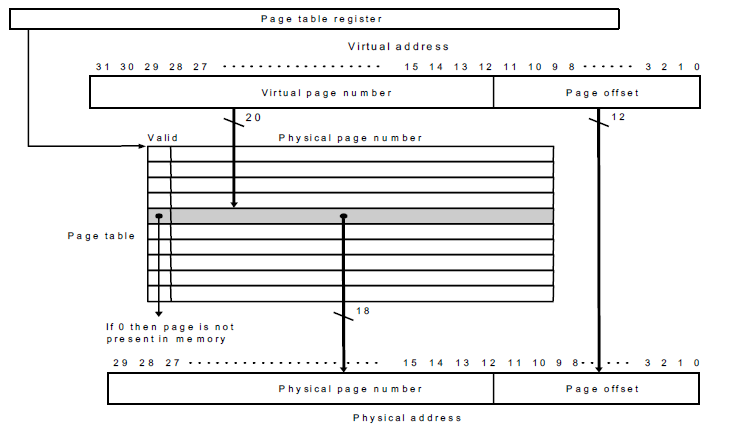
\includegraphics[width=0.42\textwidth]{CO5/Page Table Diagram}
    \caption{Page Table Diagram}
\end{figure}

\subsubsection{Page Faults}
If the valid bit for a virtual page is off, a page fault occur. 

When a page fault occurs
\begin{enumerate}\small
    \item The OS will find the page in the disk by the page table. 
    \item The OS will bring the requested page into main memory. If all the pages in main memory are in use, the OS will use LRU strategy to choose a page to replace. 
\end{enumerate}

\paragraph{How large page table?}
Assume:
\begin{itemize}\small
    \item Virtual address is 32 bits
    \item page size is 4KB
    \item Entry size is 4 bytes
\end{itemize}{\small
    \begin{align*}
        \text{Number of page table entries}&=\frac{2^{32}}{2^{12}}=2^{20}\\
        \text{Size of page table}&=2^{20}\times 2^2=4MB
    \end{align*}
}

\subsubsection{Making Address Translation Fast--TLB}
Virtual memory system must use write-back strategy. 

\paragraph{Translation-lookaside Buffer(TLB)}
The TLB acts as Cache on the page table. A cache for address translations: translation look aside buffer. 

\begin{figure}[!htb]
    \centering
    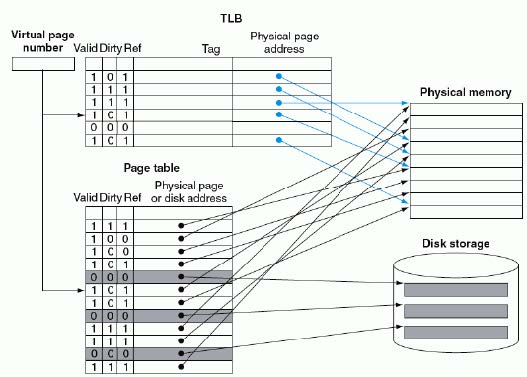
\includegraphics[width=0.42\textwidth]{CO5/Translation-lookaside Buffer}
    \caption{Translation-lookaside Buffer}
\end{figure}

\begin{figure}[!htb]
    \centering
    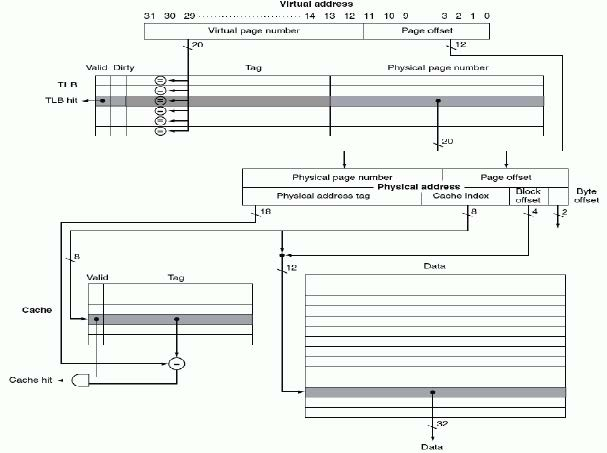
\includegraphics[width=0.42\textwidth]{CO5/FastMATH Memory Hierarchy}
    \caption{FastMATH Memory Hierarchy}
\end{figure}

\begin{figure}[!htb]
    \centering
    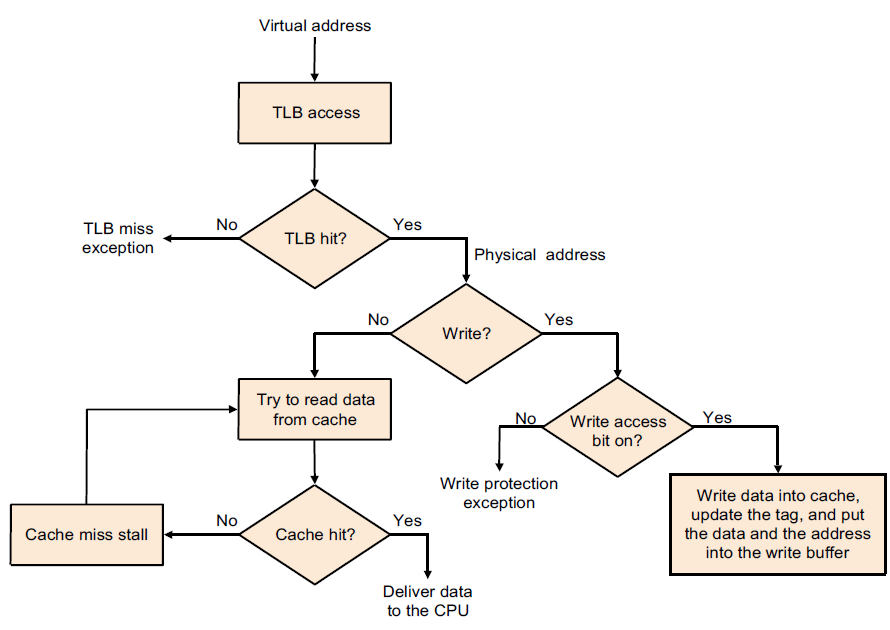
\includegraphics[width=0.42\textwidth]{CO5/TLBs and caches}
    \caption{TLBs and caches}
\end{figure}


\subsection{Possible combinations of Event}
Three different types of misses: TLB miss, page Fault, cache miss. 
\begin{figure}[!htb]
    \centering
    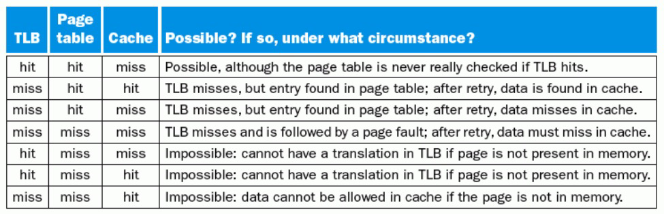
\includegraphics[width=0.42\textwidth]{CO5/Possible combinations of Event}
    \caption{Possible combinations of Event}
\end{figure}
